\begin{frame}[fragile]
\frametitle{Arrays}

    The Python \verb+list+ and \verb+dict+ objects are not suitable to manage multi-dimensional arrays. 
    \vspace{1em}

    Instead, the \href{https://numpy.org/}{Numpy} (Numerical Python) library should be used. It allows to:
    \begin{itemize}
        \item{Create multi-dimensional arrays}
        \item{Access array attributes (shape, number of dimensions, data types)}
        \item{Manipulate arrays (changing shape, tiling)}
        \item{Manipulate missing values} 
        \item{Perform optimized numerical operations (pointwise or matrix) via broadcasting (no loops)}
    \end{itemize}

    To manipulate arrays, play with the \verb+arrays.py+ file.

\end{frame}

\begin{frame}[fragile]
    \frametitle{Loops on multi-dimensional arrays}
    Computer memory is inherently linear, i.e. multi-dimensional arrays are stored in memory as one-dimensional arrays. This can be done in two ways:
    \begin{itemize}
        \item{Row-major order: C/C++, Python}
        \item{Column-major order: Fortran, Matlab, R, Julia}
    \end{itemize}

    \vspace{-1em}
    \begin{figure}
        \subfloat[Row-major order]{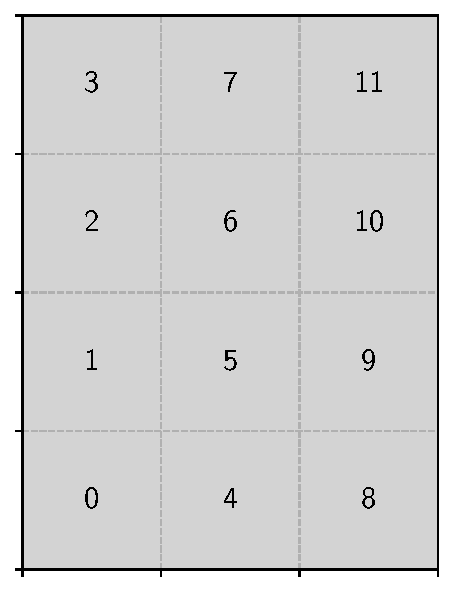
\includegraphics[scale=0.45]{figs/corder.pdf}}
        \qquad
        \subfloat[Column-major order]{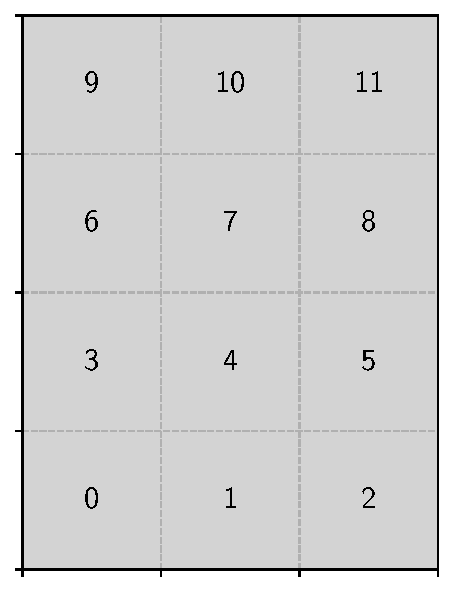
\includegraphics[scale=0.45]{figs/forder.pdf}}
    \end{figure}

\end{frame}

\begin{frame}[fragile]
    \frametitle{Loops on multi-dimensional arrays}
    Imbricated loops should be consistent with the memory ordering:

    \lstinputlisting[basicstyle=\ttfamily\scriptsize, caption={Row-order (Python)}]{scripts/loop.py}
    \lstinputlisting[basicstyle=\ttfamily\scriptsize,caption={Column-order (Julia)}, language=julia]{scripts/loop.jl}
    \vspace{1em}

    Sources: \href{https://en.wikipedia.org/wiki/Row-_and_column-major_order}{Wikipedia}, \href{https://eli.thegreenplace.net/2015/memory-layout-of-multi-dimensional-arrays/}{thegreenplace}

\end{frame}
